\documentclass[12pt, %
openright, 
oneside, %
%twoside, %TCC: Se seu texto tem mais de 100 páginas, descomente esta linha e comente a anterior
a4paper,    %
%english,   %
brazil]{facom-ufu-abntex2}


\usepackage{graphicx}
\graphicspath{{figuras/}{pictures/}{images/}{./}} % where to search for the images

\newcommand{\blue}[1]{\textcolor{blue}{#1}}
\newcommand{\red}[1]{\textcolor{red}{#1}}

%--------------Pacotes de citações
\usepackage[brazilian,hyperpageref]{backref}	 % Paginas com as citações na bibl
\usepackage[alf]{abntex2cite}	% Citações padrão ABNT

\usepackage{hyperref}


\autor{José Lucas Ferreira de Lima} %TCC
\data{2025}
\orientador{Ronaldo Castro de Oliveira} %TCC
%\coorientador{Algum?} %TCC

% ---
% Informações de dados para CAPA e FOLHA DE ROSTO
% ---

\titulo{De voltas rápidas a decisões rápidas: o processo de coleta e tratamento de dados em tempo real na Fórmula 1} %TCC

\hypersetup{pdfkeywords={Big Data, Fórmula 1, telemetria, análise de dados, Kafka, UDP, Python, dashboard, machine learning, simulação, mensageria}}

\begin{document} 
\frenchspacing 

% ----------------------------------------------------------
% ELEMENTOS PRÉ-TEXTUAIS
% ----------------------------------------------------------
%\pretextual
\imprimircapa
\imprimirfolhaderosto


% ---
% Inserir folha de aprovação
% ---
%
% \includepdf{folhadeaprovacao_final.pdf} %TCC: depois de aprovado o trabalho, descomente esta linha e comente o próximo bloco para incluir scan da folha de aprovação.
%
\begin{folhadeaprovacao}

  \begin{center}
    {\ABNTEXchapterfont\large\imprimirautor}

    \vspace*{\fill}\vspace*{\fill}
    {\ABNTEXchapterfont\bfseries\Large\imprimirtitulo}
    \vspace*{\fill}
    
    \hspace{.45\textwidth}
    \begin{minipage}{.5\textwidth}
        \imprimirpreambulo
    \end{minipage}%
    \vspace*{\fill}
   \end{center}
    
   Trabalho aprovado. \imprimirlocal, 01 de novembro de 2016: %TCC:

   \assinatura{\textbf{\imprimirorientador} \\ Orientador}  
   \assinatura{\textbf{Professor}}% \\ Convidado 1} %TCC:
   \assinatura{\textbf{Professor}}% \\ Convidado 2} %TCC:
   %\assinatura{\textbf{Professor} \\ Convidado 3}
   %\assinatura{\textbf{Professor} \\ Convidado 4}
      
   \begin{center}
    \vspace*{0.5cm}
    {\large\imprimirlocal}
    \par
    {\large\imprimirdata}
    \vspace*{1cm}
  \end{center}
  
\end{folhadeaprovacao}
% ---


%%As seções dedicatória, agradecimento e epígrafe não são obrigatórias.
%%Só as mantenha se achar pertinente.

% ---
% Dedicatória
% ---
\begin{dedicatoria}
   \vspace*{\fill}
   \centering
   \noindent
   \textit{Dedico este trabalho aos meus pais, pelo apoio incondicional em toda a minha trajetória; aos meus amigos, 
   que foram pilares essenciais durante minha jornada acadêmica; e à minha avó, que nos deixou enquanto eu construía este trabalho, 
   mas cuja memória permanece viva em meu coração.}  %TCC:
   \vspace*{\fill}
\end{dedicatoria}
% ---

% ---
% Agradecimentos
% ---
%\begin{agradecimentos}
%Agradeço a \lipsum[30]. %TCC:
%\end{agradecimentos}
% ---

% ---
% Epígrafe
% ---
%\begin{epigrafe}
%    \vspace*{\fill}
%	\begin{flushright}
%		\textit{``Alguma citação que ache conveniente? \lipsum[10]''} %TCC:
%	\end{flushright}
%\end{epigrafe}
% ---



\begin{resumo} %TCC:

  AJUSTAR AO FINAL DA ESCRITA DO TRABALHO

  A Fórmula 1 é um ambiente altamente tecnológico onde a análise de dados em 
  tempo real desempenha um papel crucial no desempenho das equipes, deixando a competitividade do esporte
  cada vez mais alta. Este trabalho explora a aplicação de \textbf{Big Data} na Fórmula 1, abordando tanto os conceitos teóricos 
  quanto uma implementação prática baseada na telemetria do jogo \textbf{F1 23}.
  
  O objetivo principal é demonstrar como a coleta e análise de dados podem fornecer insights valiosos para 
  a tomada de decisões estratégicas durante uma corrida. Para isso, foi desenvolvida uma aplicação em \textbf{Python} 
  que se conecta ao jogo pela rede local, estabelece um \textbf{socket} com este, recebe os dados de telemetria via \textbf{UDP}, 
  processa as informações, e envia os dados por mensageria utilizando \textbf{Kafka}. Os resultados são exibidos em um 
  \textbf{dashboard interativo} conectado a essa fila, permitindo análises em tempo real durante a corrida. 
  A aplicação foi testada em um ambiente controlado, e os resultados obtidos são discutidos em detalhes.
  
  A metodologia adotada inclui o estudo dos princípios do \textbf{Big Data} aplicados à F1, bem como o desenvolvimento 
  da pipeline de dados para captura e visualização dos dados do jogo. A implementação prática busca simular a experiência 
  real das equipes de F1 no uso de dados para análise de desempenho, ou seja, a visão do engenheiro de corrida durante a prova.

  Os resultados esperados incluem a demonstração do impacto do Big Data na performance das equipes e a 
  validação do potencial da tecnologia utilizada para fins de simulação e aprendizado. Este trabalho contribui 
  para a compreensão do uso da telemetria na F1 e reforça a importância da análise de dados em cenários de alta performance.

 \vspace{\onelineskip}
    
 \noindent
 \textbf{Palavras-chave}: big data, formula 1, engenharia de dados, python, pipeline. %TCC:
\end{resumo}

% ---
% inserir lista de ilustrações
% ---
\pdfbookmark[0]{\listfigurename}{lof}
\listoffigures*
\cleardoublepage
% ---

% ---
% inserir lista de tabelas
% ---
\pdfbookmark[0]{\listtablename}{lot}
\listoftables*
\cleardoublepage
% ---



% ---
% inserir lista de abreviaturas e siglas
% ---
\begin{siglas} %TCC:
  \item[Fig.] Area of the $i^{th}$ component
  \item[UDP] User Datagram Protocol
  \item[ETL] Extract, Transform, Load 
  \item[CFD] Computational Fluid Dynamics
\end{siglas}
% ---

%% ---
%% inserir lista de símbolos, se for adequado ao trabalho. %TCC:
%% ---
%\begin{simbolos}
%  \item[$ \Gamma $] Letra grega Gama
%  \item[$ \Lambda $] Lambda
%  \item[$ \zeta $] Letra grega minúscula zeta
%  \item[$ \in $] Pertence
%\end{simbolos}
%% ---

% ---
% inserir o sumario
% ---
\pdfbookmark[0]{\contentsname}{toc}
\tableofcontents*
\cleardoublepage
% ---





% ----------------------------------------------------------
% ELEMENTOS TEXTUAIS
% ----------------------------------------------------------
\textual


% ----------------------------------------------------------
% Introdução
% ----------------------------------------------------------

\chapter[Introdução]{Introdução}
%TCC:
\section{Contextualização e Motivação}

De acordo com um artigo publicado pela \citeonline{Mercedes}, cada carro de Fórmula 1 é equipado com
mais de 250 sensores categorizados em controle, instrumentação e monitoramento, 
que coletam dados vitais de pressão, temperatura, inércia e deslocamento de todos os 
sistemas do veículo. Durante um fim de semana de corrida, o volume total de dados 
gerados por um único carro, incluindo telemetria ao vivo (cerca de 30 MB por volta), 
vídeo e informações auxiliares, excede 1 terabyte, podendo duplicar ou triplicar após 
o pós-processamento. Adicionalmente, as fábricas contribuem com vasta quantidade de 
dados provenientes de dinamômetros, simuladores e túneis de vento, criando um 
ecossistema de informação que exige a transferência de até 11 terabytes entre a pista 
e as sedes em Brackley e Brixworth, com telemetria ao vivo chegando em meros 10 
milissegundos em corridas europeias. Essa imensa e contínua geração de dados sublinha 
a natureza intensiva em dados da Fórmula 1 moderna.

No cenário altamente competitivo da Fórmula 1, a premissa fundamental é que a 
ciência de dados, e por extensão, a otimização da performance, não pode existir sem 
um fluxo contínuo e confiável de informações. A limitação drástica do tempo de testes 
em pista impõe uma pressão imensa para a coleta de dados precisos e completos na 
primeira tentativa, pois não há oportunidade para repetições, como aponta a 
\citeonline{Mercedes}. Essa característica ressalta a importância crítica de 
uma infraestrutura de dados robusta, onde, como detalhado por \citeonline{Msakamali}, a 
análise de dados é fundamental para aprimorar o desempenho e embasar decisões 
estratégicas em tempo real. Uma vez coletados do carro, os dados são sincronizados, 
criptografados e transmitidos via telemetria para a garagem, garantindo que engenheiros
e pilotos tenham acesso a informações consistentes e seguras. O uso de software 
especializado, como o ATLAS da McLaren Applied, tanto em tempo real quanto para 
análises retrospectivas, demonstra a dedicação contínua à extração de insights valiosos,
seja para comparar o desempenho dos pilotos, analisar dados de frenagem e velocidades 
de curva, ou para identificar oportunidades que tornarão o carro e o piloto ainda mais 
rápidos. A enorme quantidade de dados, embora desafiadora, é também uma oportunidade de 
engenharia para priorizar e analisar as informações corretas, acelerando o aprendizado 
e a evolução das equipes. Assim, a existência de uma pipeline de coleta e processamento 
de dados em tempo real não é apenas uma conveniência, mas uma necessidade estratégica e 
operacional para sustentar a competitividade na Fórmula 1.

A competitividade na Fórmula 1 moderna é diretamente proporcional à confiabilidade dos 
dados, pois a ciência e a tomada de decisão dependem intrinsecamente da qualidade e 
integridade da informação. Dados imprecisos ou inconsistentes comprometem insights e 
decisões estratégicas, como enfatizado por \citeonline{Suman}. Em um ambiente de alta 
performance e tempo crítico, a latência é inaceitável; a transformação de vastos volumes
de telemetria em conhecimento acionável em milissegundos exige uma arquitetura de dados 
eficiente. O processamento em tempo real, segundo o artigo do \citeonline{Estuary}, é crucial para insights 
imediatos e ações ágeis, permitindo a detecção e correção de anomalias. Assim, torna-se 
imperativa uma pipeline robusta de coleta, transmissão e processamento em tempo real, 
capaz de assegurar a integridade e prontidão dos dados do sensor até o engenheiro, 
garantindo resultados críveis e reproduzíveis \cite{SciSure}.

Diante da complexidade e da criticidade dos desafios impostos pela volumosa geração e 
pela necessidade de processamento em tempo real dos dados na Fórmula 1, este trabalho 
propõe uma solução prática e inovadora. Nosso estudo se dedicará a explorar e aplicar 
diversas técnicas de ETL (Extract, Transform, Load) para construir uma pipeline robusta,
tolerante a falhas e escalável de coleta e processamento de dados. O diferencial reside 
na utilização de ferramentas gratuitas e open-source, demonstrando que é possível 
desenvolver soluções de alta performance e segurança sem depender de softwares 
proprietários ou de alto custo. O objetivo é evidenciar como essas tecnologias podem 
efetivamente resolver o problema da aquisição, tratamento e disponibilização dos 
terabytes de dados gerados, garantindo que as equipes de Fórmula 1 possam extrair 
insights valiosos e tomar decisões ainda mais assertivas em um ambiente onde cada 
milissegundo conta.

\section{Problema de Pesquisa}

A Fórmula 1 contemporânea, impulsionada por uma colossal geração de dados – com mais de 
250 sensores em cada carro produzindo terabytes de informações cruciais por fim de semana
de corrida –, demanda uma capacidade sem precedentes de coleta, processamento e análise 
em tempo real para a otimização contínua do desempenho das equipes. Diante desse cenário 
de alta complexidade e criticidade temporal, surge o seguinte problema de pesquisa:

- Como é possível projetar e implementar uma pipeline de dados robusta, tolerante a 
falhas e escalável, utilizando tecnologias modernas, preferencialmente open-source, que 
garanta a extração, transporte (com mínima latência, integridade e segurança), 
transformação de valores brutos em formatos legíveis e a visualização efetiva de 
terabytes de dados provenientes de múltiplos sensores veiculares da Fórmula 1, tudo 
isso no menor espaço de tempo possível, para subsidiar decisões estratégicas e 
operacionais das equipes?

Este trabalho se propõe a responder a essa questão fundamental, explorando a aplicação 
de técnicas de ETL (Extract, Transform, Load) e arquiteturas de processamento de stream 
de dados, visando demonstrar a viabilidade de construir uma solução eficiente e segura 
para o ecossistema de dados da Fórmula 1.

\section{Objetivos}
\subsection{Objetivo Geral}

O objetivo geral deste trabalho é projetar e implementar uma pipeline de dados em larga 
escala, robusta e eficiente, utilizando exclusivamente softwares de código aberto, para
simular o processo completo de coleta e tratamento de dados em tempo real no contexto da 
Fórmula 1. Esta pipeline servirá como um alicerce fundamental para futuras aplicações de 
ciência de dados e inteligência artificial, demonstrando a viabilidade de transformar 
volumes massivos de dados brutos em informações acionáveis para otimizar a performance.

\subsection{Objetivos Específicos}

Alguns objetivos específicos deste trabalho incluem:

\begin{itemize}
  \item \textbf{Analisar os Conceitos de ETL e Processamento de Dados em Tempo Real}: Investigar 
  e compreender os principais conceitos de Extração, Transformação e Carga (ETL), 
  bem como as metodologias de processamento de dados em tempo real (streaming), 
  focando em sua aplicabilidade e desafios em ambientes de alta velocidade e volumetria 
  de dados, como a Fórmula 1.
  \item \textbf{Desenvolver um Módulo de Coleta e Pré-processamento de Telemetria}: Criar uma 
  aplicação em Python capaz de estabelecer conexão com uma fonte simulada de dados de 
  telemetria da Fórmula 1 (neste caso, o jogo F1 23), realizar a extração e o pré-processamento inicial desses 
  dados (transformação de valores binários/brutos para formatos legíveis), e 
  encaminhá-los para um sistema de mensageria.
  \item \textbf{Implementar uma Arquitetura de Mensageria e Processamento de Streams}: Configurar 
  e integrar um sistema de mensageria (message broker) para garantir a transmissão 
  eficiente e tolerante a falhas dos dados, e desenvolver módulos de processamento que 
  consumam esses dados em tempo real, aplicando transformações e enriquecimentos 
  necessários.
  \item \textbf{Visualizar Dados de Telemetria em Tempo Real}: Construir um dashboard 
  interativo que receba os dados processados e os exiba graficamente em tempo real, 
  permitindo a visualização clara de métricas cruciais de desempenho veicular, validando 
  a funcionalidade e a latência da pipeline.
  \item \textbf{Avaliar a Eficiência e a Robustez da Pipeline}: Realizar testes controlados 
  na aplicação desenvolvida para analisar o desempenho da pipeline em termos de latência, 
  vazão (throughput), integridade dos dados e tolerância a falhas, utilizando métricas 
  quantitativas.
  \item \textbf{Discutir Implicações e Aplicações Futuras da Ciência de Dados}: Apresentar 
  como os dados coletados e processados podem subsidiar a tomada de decisões estratégicas 
  por engenheiros na Fórmula 1 e propor futuras melhorias e extensões para a pipeline 
  desenvolvida, incluindo potencial integração com modelos de ciência de dados e 
  inteligência artificial.
\end{itemize}

\section{Justificativa}

A Fórmula 1, mais do que um esporte de alta velocidade, consolidou-se como um dos 
ecossistemas mais avançados para o estudo e aplicação da engenharia e ciência de dados. 
Cada carro é, em essência, um laboratório de inovação em tempo real, equipado para gerar 
uma quantidade colossal de informações – com dados de telemetria que podem chegar a 1,5 
terabytes por fim de semana de corrida \cite{Luzich}. Conforme evidenciado por 
\citeonline{Msakamali}, a análise de dados na F1 é fundamental para aprimorar o desempenho na corrida, 
fornecendo uma base sólida para a tomada de decisões estratégicas em tempo real. 
Nesse ambiente, a tecnologia de dados não é apenas um suporte, mas um diferencial estratégico crucial, 
tornando a F1 um campo de estudo exemplar para desafios contemporâneos em processamento de streaming e engenharia de 
dados de alta performance.

Apesar do vasto potencial dos dados na Fórmula 1, sua exploração plena é barrada por 
desafios técnicos inerentes ao Big Data, especialmente a velocidade e o volume com que 
são gerados. Cada milissegundo de atraso na aquisição ou processamento de dados pode 
comprometer uma decisão estratégica, tornando a baixa latência um requisito não 
negociável. Conforme a \citeonline{Mercedes} destaca, a transmissão de 
telemetria em tempo real, embora impressionantemente rápida (10 milissegundos em 
corridas europeias), ainda lida com a complexidade de milhões de pontos de dados por 
segundo. Além da velocidade, a variedade dos dados provenientes de centenas de sensores 
exige sistemas que possam integrar e harmonizar diferentes formatos e estruturas. Tais 
complexidades impõem a necessidade crítica de pipelines de dados robustas, eficientes e 
seguras. Essas pipelines não apenas garantem a coleta e o transporte ininterrupto das 
informações, mas também realizam as transformações necessárias para converter dados 
brutos em insights acionáveis, salvaguardando a integridade e a segurança da informação 
desde o carro até a tomada de decisão final.

Para além do espetáculo e da competitividade da pista, os avanços tecnológicos e as 
soluções desenvolvidas na Fórmula 1, particularmente no que tange à engenharia de dados 
e processamento em tempo real, possuem um impacto e uma aplicabilidade notáveis em 
diversos outros setores. Os desafios de gerenciar volume massivo, alta velocidade, 
variedade de dados e a necessidade de baixa latência – inerentes ao ambiente da F1 – 
são, em essência, os mesmos enfrentados pela indústria moderna, especialmente no 
contexto da Indústria 4.0 \cite{Singh2021BigData}. Setores como a manufatura, 
por exemplo, demandam a capacidade de coletar e processar dados de sensores em tempo 
real para fins de manutenção preditiva, otimização de linhas de produção e controle de 
qualidade, onde cada milissegundo na detecção de anomalias pode significar uma economia 
substancial ou a prevenção de falhas catastróficas \cite{Wijesinghe2024Predictive}. 
Dessa forma, o estudo aprofundado dos processos de coleta e tratamento de dados em tempo 
real na Fórmula 1 não apenas revela as inovações de ponta da categoria, mas também serve 
como um modelo prático e um campo de testes para demonstrar como a engenharia de dados 
e o Big Data podem ser aliados estratégicos fundamentais na tomada de decisões em 
cenários de alta performance e complexidade industrial.

\section{Metodologia do Trabalho}

Esta seção detalha o planejamento e a execução do desenvolvimento da pipeline de dados em tempo real para simular o processo de coleta e tratamento de telemetria na Fórmula 1.

\subsection{Tipo e Abordagem da Pesquisa}
O presente trabalho classifica-se como uma pesquisa de natureza \textbf{aplicada}, pois visa desenvolver e implementar uma solução prática para um problema real na engenharia de dados. A abordagem é predominantemente \textbf{quantitativa} e \textbf{experimental}, centrada na construção, validação e análise de desempenho de uma arquitetura de pipeline de dados em tempo real, utilizando métricas objetivas como latência e \textit{throughput}.

\subsection{Desenho da Solução: Arquitetura da Pipeline}
Para atingir os objetivos propostos, será desenvolvida uma arquitetura de pipeline de dados \textit{end-to-end} conforme ilustrado na Figura \ref{fig:arquitetura}.

\begin{figure}[h!]
    \centering
    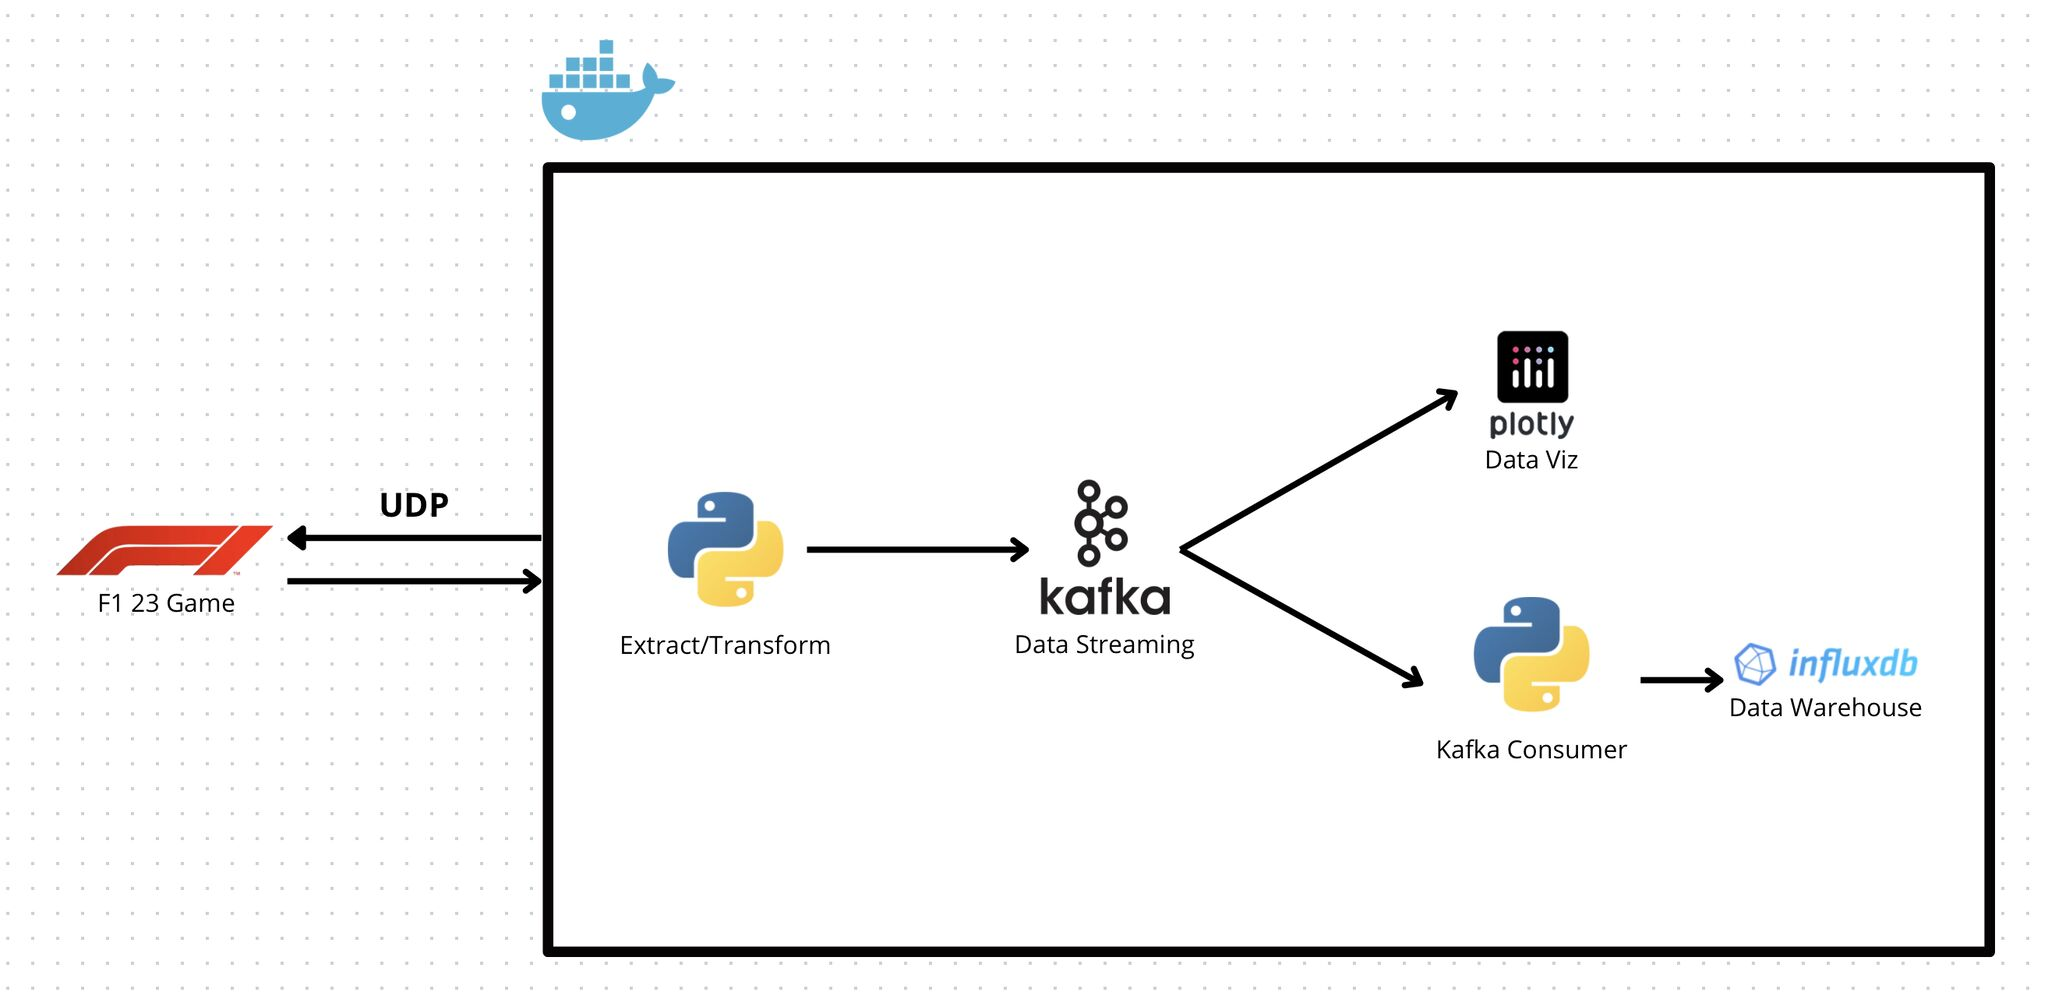
\includegraphics[width=0.9\textwidth]{1744514910436.jpeg}
    \caption{Arquitetura Proposta da Pipeline de Dados}
    \label{fig:arquitetura}
\end{figure}

A arquitetura proposta compreende os seguintes módulos e fluxo de dados:
\begin{itemize}
    \item \textbf{Fonte de Dados:} O jogo \textbf{F1 23} será utilizado como a fonte primária para simular a geração de dados de telemetria em tempo real, transmitindo-os via protocolo \textbf{UDP (User Datagram Protocol)}.
    \item \textbf{Módulo de Extração/Transformação (Python):} Uma aplicação desenvolvida em \textbf{Python} será responsável por capturar os dados UDP brutos do jogo. Este módulo realizará a etapa de \textbf{Extração}, lendo os pacotes de dados, e a primeira fase de \textbf{Transformação}, convertendo os valores binários recebidos em formatos legíveis (inteiros e decimais) e estruturando-os para processamento.
    \item \textbf{Mensageria (Kafka):} Após a extração e transformação inicial, os dados serão publicados em tópicos do \textbf{Apache Kafka}, servindo como uma plataforma de \textit{streaming} de dados. O Kafka garantirá a transmissão eficiente, tolerante a falhas e escalável dos dados em tempo real.
    \item \textbf{Consumo e Persistência (Kafka Consumer / InfluxDB):} Um segundo módulo em \textbf{Python} atuará como \textbf{Kafka Consumer}, lendo os dados dos tópicos do Kafka. Este consumidor será responsável por carregar os dados em um \textbf{InfluxDB}, que funcionará como um \textit{Data Warehouse} especializado em séries temporais, permitindo o armazenamento e a recuperação eficiente de grandes volumes de dados de telemetria.
    \item \textbf{Visualização (Plotly/Dash):} Para a visualização em tempo real, um \textit{dashboard} interativo será desenvolvido utilizando a biblioteca \textbf{Dash} (baseada em Plotly). Este \textit{dashboard} consumirá os dados diretamente dos tópicos do Kafka, exibindo as métricas processadas em tempo real e fornecendo uma interface visual para acompanhamento e análise.
\end{itemize}

\subsection{Ferramentas e Tecnologias Utilizadas}
Para a implementação da pipeline, serão utilizadas as seguintes tecnologias de código aberto:
\begin{itemize}
    \item \textbf{Linguagem de Programação:} Python (para os módulos de extração/transformação e consumo/persistência).
    \item \textbf{Orquestração de Contêineres:} Docker ou Podman (para empacotar e gerenciar os serviços da pipeline, como Kafka e InfluxDB).
    \item \textbf{Plataforma de Streaming de Dados:} Apache Kafka.
    \item \textbf{Banco de Dados de Séries Temporais:} InfluxDB.
    \item \textbf{Framework para Dashboards Interativos:} Dash (com Plotly para visualização de dados).
    \item \textbf{Fonte de Dados de Telemetria:} Jogo F1 23.
\end{itemize}

\subsection{Procedimentos de Desenvolvimento}
A construção da pipeline seguirá as seguintes etapas interconectadas:
\begin{enumerate}
    \item \textbf{Configuração do Ambiente:} Preparação do ambiente de desenvolvimento, incluindo a instalação de Docker/Podman e a configuração dos contêineres para Kafka e InfluxDB.
    \item \textbf{Módulo de Extração e Transformação:} Desenvolvimento do script Python para capturar dados UDP do F1 23, realizar o \textit{parsing} inicial dos pacotes de telemetria e publicar os dados processados no Kafka.
    \item \textbf{Módulo de Persistência:} Implementação do script Python \texttt{Kafka Consumer} que consumirá os dados do Kafka e os armazenará no InfluxDB.
    \item \textbf{Módulo de Visualização:} Desenvolvimento do \textit{dashboard} interativo com Dash/Plotly, configurando-o para consumir dados em tempo real diretamente do Kafka e exibir as métricas de telemetria relevantes.
    \item \textbf{Integração e Testes Iniciais:} Conexão e validação de todos os módulos da pipeline em conjunto para assegurar o fluxo de dados contínuo e correto.
\end{enumerate}

\subsection{Estratégias de Avaliação e Validação}
A robustez e a eficiência da pipeline serão avaliadas através de testes sistemáticos, focando nas seguintes métricas e aspectos:
\begin{itemize}
    \item \textbf{Tempo de Processamento (Latência):} Medição do tempo desde a geração do dado no jogo F1 23 até sua visualização no \textit{dashboard} e persistência no InfluxDB.
    \item \textbf{Taxa de Perda de Pacotes:} Verificação da integridade do fluxo de dados para identificar qualquer perda de informação durante a transmissão e o processamento.
    \item \textbf{Volume/Stress:} Testes de carga para avaliar o desempenho da pipeline sob diferentes volumes de dados, simulando cenários de alta demanda.
    \item \textbf{Integridade dos Dados:} Validação da consistência e precisão dos dados após as etapas de transformação, comparando-os com os dados brutos da fonte.
    \item \textbf{Funcionalidade do Dashboard:} Verificação da correta exibição e atualização das métricas no \textit{dashboard}, garantindo sua usabilidade para a análise de dados em tempo real.
    \item \textbf{Diferentes Condições de Pista:} Simulação de cenários variados no jogo F1 23 para testar a adaptabilidade da pipeline a diferentes tipos e volumes de dados gerados (ex: chuva, trechos de alta/baixa velocidade).
\end{itemize}

\section{Estrutura do Trabalho}

Este trabalho está organizado em cinco capítulos principais, cada um abordando um 
aspecto fundamental da pesquisa sobre o processo de coleta e tratamento de dados em 
tempo real na Fórmula 1, desde a contextualização teórica e a metodologia de engenharia 
de dados até a análise dos resultados obtidos.

No \textbf{Capítulo 1 - Introdução}, são apresentados o tema da pesquisa, a 
contextualização e motivação para o estudo, que destaca a evolução da Fórmula 1 para um 
esporte intensivo em dados, bem como a formulação do problema de pesquisa. Além disso, 
são definidos os objetivos geral e específicos, a justificativa para a escolha do tema 
e a relevância do estudo. Também são descritos a metodologia utilizada e a própria 
estrutura do trabalho.

O \textbf{Capítulo 2 - Revisão Bibliográfica} traz um embasamento teórico sobre os 
conceitos fundamentais de engenharia de dados, processamento de dados em tempo real 
(streaming) e Extração, Transformação e Carga (ETL), e sua aplicação no contexto da 
Fórmula 1. São abordados temas como a telemetria e a coleta massiva de dados em tempo 
real na categoria, além das principais tecnologias utilizadas na construção de 
pipelines de dados, incluindo Python, Apache Kafka, Docker/Podman e InfluxDB. Este 
capítulo também inclui uma revisão de trabalhos relacionados e uma discussão sobre a 
indispensabilidade da engenharia de dados para a otimização da performance na F1.

No \textbf{Capítulo 3 - Desenvolvimento}, são detalhados os aspectos técnicos e práticos 
do estudo. Este capítulo apresenta a arquitetura da solução proposta para a pipeline de 
dados, os métodos específicos de extração de dados via telemetria simulada do jogo F1 23, 
e os processos de transformação, mensageria e armazenamento dessas informações. Além 
disso, aborda-se a implementação do dashboard interativo para visualização dos dados em 
tempo real e os testes realizados para validação prática da solução.

O \textbf{Capítulo 4 - Análise dos Resultados} apresenta a avaliação detalhada da 
pipeline desenvolvida, discutindo seu desempenho e eficiência em termos de latência, 
throughput, integridade dos dados e robustez sob diferentes condições. Também são 
analisadas as limitações do estudo e possíveis melhorias futuras que podem ser 
implementadas para aprimorar os processos investigados.

Por fim, o \textbf{Capítulo 5 - Conclusão e Trabalhos Futuros} revisita os objetivos 
propostos no início do trabalho e discute as principais contribuições da pesquisa para a 
área de engenharia de dados em tempo real. São destacados os desafios encontrados ao 
longo do estudo e sugeridas aplicações futuras para os conceitos e tecnologias exploradas, 
considerando possíveis avanços na área e a expansão da pipeline.

% ---
% Revisão Bibliográfica
% ---

\chapter{Revisão Bibliográfica}
%TCC:
\section{Engenharia de dados}
A Engenharia de Dados é uma disciplina fundamental no cenário atual da informação, atuando como a 
espinha dorsal para a criação de valor a partir de grandes volumes de dados. 
Ela se concentra no projeto, construção, otimização e manutenção de infraestruturas e sistemas 
para a coleta, processamento, armazenamento e disponibilização de dados de forma eficiente e 
confiável \cite{Reis2022DataEngineering}. Esta área abrange uma gama de atividades que vão desde a 
ingestão e limpeza de dados até a sua transformação e modelagem, preparando-os para análises 
subsequentes e para o consumo por analistas, cientistas de dados e algoritmos de machine learning. 
Seu objetivo primordial é garantir a qualidade, integridade, segurança e acessibilidade dos dados, 
permitindo que as organizações derivem insights precisos e automatizem processos decisórios.

No contexto da Fórmula 1, a Engenharia de Dados assume um papel ainda mais crítico, dada a 
exigência por dados em tempo real e de alta fidelidade. Ela é indispensável para a criação de 
pipelines robustas e confiáveis que extraiam terabytes de dados brutos dos sensores veiculares, os 
transformem em informações úteis e os armazenem de forma escalável e segura. Essa infraestrutura 
de dados assegura que engenheiros e estrategistas no pit wall e na fábrica possam acessar as 
informações necessárias com mínima latência, possibilitando tomadas de decisão estratégicas e 
operacionais em frações de segundo durante as sessões de treino, qualificação e corrida. Além 
disso, a Engenharia de Dados é a responsável por mitigar desafios como perda de pacotes, corrupção 
de dados e inconsistências, garantindo a integridade e a confiabilidade que são cruciais para a 
vantagem competitiva na F1.

\section{Análise de dados}

A análise de dados é uma etapa fundamental para a extração de insights e tomada de decisões estratégicas. Ela envolve a coleta, processamento, modelagem e interpretação de dados para identificar padrões, tendências e correlações relevantes,
envolvendo massivamente a utilização de técnicas de estatística, matemática avançada, machine learning e visualização de dados.
Na Fórmula 1, a análise de dados é utilizada para monitorar o desempenho dos carros, simular cenários de corrida, prever resultados e otimizar estratégias de corrida.

Ao longo deste trabalho, iremos discutir sobre a sua importância ao final do fluxo dos dados, afinal, de nada adianta coletar, processar e armazenar os dados se não conseguirmos extrair valor deles. Para isso, utilizaremos técnicas de visualização de dados, como
análise exploratória, gráficos e dashboards, para facilitar a interpretação dos dados e a tomada de decisões.

\section{Conceitos fundamentais de dados em tempo real (streaming)}

No panorama atual da ciência de dados, a capacidade de processar informações em tempo hábil 
tornou-se um diferencial competitivo crucial para organizações e sistemas complexos. 
Tradicionalmente, o processamento de dados era predominantemente realizado em modo de lote 
(\textit{batch processing}), onde grandes volumes de dados são coletados e processados 
periodicamente. Embora eficiente para tarefas que não exigem imediatismo, essa abordagem apresenta 
limitações significativas em cenários dinâmicos e de alta volatilidade \cite{Hashem2015BigData}.

É nesse contexto que o processamento de dados em tempo real (\textit{real-time data processing}), 
ou \textit{streaming} de dados, emerge como uma abordagem indispensável. O \textit{streaming} de 
dados refere-se à metodologia de processamento de informações à medida que elas são geradas ou chegam, 
de forma contínua e com mínima latência \cite{Xu2018RealTime}. Diferentemente do 
processamento em lote, que opera sobre conjuntos de dados estáticos e finitos, o processamento 
de \textit{streaming} lida com fluxos de dados contínuos e potencialmente ilimitados.

As principais características que definem o processamento de \textit{streaming} incluem:
\begin{itemize}
\item \textbf{Baixa Latência:} A informação é processada e disponibilizada com o menor atraso possível, frequentemente na ordem de milissegundos, o que é vital para tomadas de decisão ágeis.
\item \textbf{Processamento Contínuo:} Os dados são consumidos e processados incessantemente, sem interrupções ou a necessidade de acumular grandes volumes antes da análise.
\item \textbf{Alta Velocidade e Volume:} Os sistemas de \textit{streaming} são projetados para gerenciar e analisar grandes volumes de dados que chegam em taxas extremamente elevadas.
\end{itemize}

A relevância do processamento de \textit{streaming} é particularmente acentuada em domínios como a 
Fórmula 1. Dada a criticidade do tempo em decisões estratégicas – como ajustes de performance 
veicular, gestão de pneus ou respostas a incidentes em pista – a análise instantânea dos dados de 
telemetria provenientes de centenas de sensores é fundamental. A capacidade de processar e reagir 
a esses fluxos contínuos de dados permite que as equipes otimizem o desempenho em frações de 
segundo, transformando a agilidade informacional em vantagem competitiva \cite{Mercedes}.

\section{Extração, Transformação e Carga (ETL)}
Segundo \citeonline{Seenivasan2023ETL}, estes trabalhos são responsáveis pela extração de dados
de diversas fontes (no nosso caso, os sensores do carro), transformação desses dados para torná-los mais
consistentes e úteis, e carregamento desses dados em um sistema de armazenamento (como um banco de dados ou \textit{data warehouse}).

Como apontado pela \citeonline{Mercedes}, os carros possuem em torno de 250 sensores em sua construção, o que exige a construção
de uma pipeline de dados robusta e eficiente para coletar, processar e armazenar esses dados em tempo real. \citeonline{Mehmood2020Challenges} sugere que
a construção de uma pipeline de ETL em tempo real é bem desafiadora, vide a própria natureza do dado em respeito
ao seu volume, variedade, velocidade, volatilidade, variabilidade, veracidade e valor - todos esses desafios serão amplamente encontrados aqui,
já que os sensores disparam diferentes tipos de dados em formatos diferentes, num grande volume e numa velocidade
altíssima.

Sendo assim, chega-se à conclusão de que a implementação das melhores práticas de ETL tornam esse processo muito mais simples
de ser construído e permite que as equipes atingam maior vantagem competitiva.

\section{Telemetria de dados em tempo real}
O grande desafio de todas as equipes até aqui: como coletar gigabytes de dados de diversos formatos em uma rede privada, compartilhada apenas
entre as equipes, de forma segura, eficiente e no menor espaço de tempo possível, e mais, sem deixar esse dado ser corrompido ou perdido? 
O começo de tudo é a telemetria, que é a tecnologia que permite a coleta, transmissão e análise de dados em tempo real.

Todos os sensores do carro monitoram os componentes atrelados a si e, a cada milissegundo ou segundo, enviam esses dados para o paddock através de uma conexão
com um computador disponibilizado aos engenheiros de equipe. Esses dados são enviados através de uma conexão UDP, que é um protocolo de comunicação rápido e 
eficiente, ideal para a transmissão de dados em tempo real.

Assim que os dados chegam ao computador, uma pipeline de dados é acionada, que é responsável por processar, armazenar e analisar esses dados. Esse passo é necessário
pois os dados chegam em um formato de binário, que precisa ser tratado e transformado em informações úteis para os engenheiros - uma dessas
transformações é justamente converter os dados binários para inteiros e números decimais. 

A pipeline é composta por diversas etapas, como a coleta, transformação e carregamento dos dados. Com os dados já tratados, eles são enviados para um sistema de mensageria,
que é responsável por transmitir esses dados para o dashboard, que é a interface gráfica que os engenheiros utilizam para analisar o desempenho do carro em tempo real.

Além disso, podemos, também, armazenar esses dados tratados em um banco, seja ele relacional ou não, para futuras análises e consultas. Isso é importante pois,
com o passar do tempo, podemos identificar padrões e tendências que não seriam possíveis de serem identificados em tempo real. Outra possibilidade seria justamente
usar esses dados para treinar um modelo de machine learning, que pode prever o desempenho do carro em diferentes cenários, ou até mesmo simular corridas.

Com base na telemetria, os engenheiros conseguem pensar em estratégias, realizar ajustes no carro e testar o desempenho dessas modificações.
Ele também consegue monitorar o desempenho do piloto, analisando sua concentração, batimentos cardíacos e pressão sanguínea, o que pode
ajudar outros membros da equipe a fazer melhorias no treino físico do piloto, além de ajustar o carro de acordo com suas necessidades, aumentando
o conforto para que o piloto possa se concentrar apenas em pilotar.

\section{Tecnologias Utilizadas}

\subsection{Python}
Python é uma linguagem de programação de alto nível, interpretada, de script, imperativa, orientada a objetos, funcional, de tipagem dinâmica e forte.
Foi lançada por Guido van Rossum em 1991 com o objetivo de ser uma linguagem de fácil leitura e aprendizado, com uma sintaxe limpa e clara, diferentemente de C, que inspirou sua criação.
Atualmente, é uma das linguagens mais populares do mundo, com uma comunidade ativa e uma vasta quantidade de bibliotecas, tanto para desenvolvimento web, científico, como para automação de tarefas.

Neste trabalho, iremos utilizá-la para desenvolver a aplicação que se conecta ao jogo, recebe os dados de telemetria, processa esses dados e envia para a mensageria, além do dashboard final que exibirá os dados tratados.
Sua escolha se deu pela facilidade de uso, vasta quantidade de bibliotecas disponíveis e por ser uma linguagem de alto nível, o que facilita o desenvolvimento e manutenção do código.

\subsection{Kafka}
Apache Kafka é uma plataforma de mensageria distribuída, que permite a publicação e subscrição de streams de dados em tempo real. Foi criada pela LinkedIn em 2011 e, atualmente, é mantida pela Apache Software Foundation.
Sua arquitetura é baseada em tópicos, partições e consumidores, o que permite a escalabilidade e tolerância a falhas. Além disso, é altamente eficiente, sendo capaz de lidar com milhões de mensagens por segundo.

Seu uso neste trabalho será extremamente importante visto a quantidade de dados que serão gerados e a necessidade de transmiti-los em tempo real para o dashboard sem perda de informações.
Nestes casos, o Kafka é a melhor opção, pois garante a entrega das mensagens e a escalabilidade necessária para lidar com a quantidade de dados gerados.

\subsection{Docker}
Docker é uma plataforma de código aberto que facilita a criação, implantação e execução de aplicativos em contêineres. Contêineres permitem que um desenvolvedor empacote uma aplicação com todas as partes necessárias, como bibliotecas e outras dependências, e a envie como uma única imagem.
Com essa ferramenta, podemos colocar uma série de serviços em contêineres, como o Kafka, o dashboard e o banco de dados, e executá-los juntos, garantindo que todos os serviços estejam disponíveis e funcionando corretamente, facilitando a execução e o gerenciamento da aplicação,
além de garantir que a aplicação funcione da mesma forma em diferentes ambientes.

Neste trabalho, sua utilização se dá pela sua leveza, facilidade de uso e interconectividade entre as ferramentas presentes no contêiner, o que facilita a execução e o gerenciamento da aplicação.

\subsection{InfluxDB}
InfluxDB é um banco de dados de séries temporais de código aberto, otimizado para armazenar e consultar grandes volumes de dados de séries temporais em tempo real. Ele foi criado pela InfluxData em 2013 e, atualmente, é mantido pela mesma.
Sua arquitetura é baseada em séries temporais, pontos de dados e tags, o que permite a rápida inserção e consulta de dados de séries temporais. Além disso, é altamente escalável, sendo capaz de lidar com milhões de pontos de dados por segundo.

Sua utilização neste trabalho se dá pela necessidade de armazenar os dados tratados para futuras análises, consultas e alimentar modelos de inteligência artificial, 
além de garantir a integridade e a disponibilidade dos dados gerados. 

\section{Trabalhos Relacionados}

Ver com o Ronaldo depois para entender o que podemos colocar aqui.

% ---
% Desenvolvimento
% ---

\chapter{Desenvolvimento}
%TCC:
Um ou mais capítulos (por exemplo um para testes)
\section{Arquitetura da Solução}
\section{Coleta de Dados via Telemetria}
\section{Processamento e Armazenamento de Dados}
\section{Visualização dos Dados}
\section{Implementação e Testes}


\begin{figure}[!ht]
    \centering
	
\includegraphics[width=0.55\linewidth]{imagemExemplo.pdf}
	\caption[Isso é o que aparece no sumário]{Imagem de exemplo.}
	\label{fig:graficosVariandoTamanhoRede}
\end{figure}

% ---
% Análise dos Resultados
% ---

\chapter{Análise dos Resultados}
\section{Validação da Coleta e Processamento}
\section{Desempenho e Eficiência da Aplicação}
\section{Limitações e Melhorias Futuras}




%TCC:
%TCC:
%TCC:
%TCC:

% ---
% Conclusão
% ---
\chapter{Conclusão e Trabalhos Futuros}
%TCC:
E daí?
\section{Revisão dos Objetivos e Contribuições}
\section{Desafios Encontrados}
\section{Aplicações Futuras}





% ----------------------------------------------------------
% ELEMENTOS PÓS-TEXTUAIS
% ----------------------------------------------------------
\postextual


% ----------------------------------------------------------
% Referências bibliográficas
% ----------------------------------------------------------
\bibliography{ref}


%% ----------------------------------------------------------
%% Apêndices TCC: só mantenha se for pertinente.
%% ----------------------------------------------------------

% ---
% Inicia os apêndices
% ---
\begin{apendicesenv}

% Imprime uma página indicando o início dos apêndices
\partapendices

% ----------------------------------------------------------
\chapter{Quisque libero justo}
% ----------------------------------------------------------

\lipsum[50]

% ----------------------------------------------------------
\chapter{Coisas que fiz e que achei interessante mas não tanto para entrar no corpo do texto}
% ----------------------------------------------------------
\lipsum[55-57]

\end{apendicesenv}
% ---


% ----------------------------------------------------------
% Anexos %TCC: so mantenha se pertinente.
% ----------------------------------------------------------

% ---
% Inicia os anexos
% ---
\begin{anexosenv}

% Imprime uma página indicando o início dos anexos
\partanexos

% ---
\chapter{Eu sempre quis aprender latim}
% ---
\lipsum[30]

% ---
\chapter{Coisas que eu não fiz mas que achei interessante o suficiente para colocar aqui}
% ---

\lipsum[31]

% ---
\chapter{Fusce facilisis lacinia dui}
% ---

\lipsum[32]

\end{anexosenv}

%---------------------------------------------------------------------
% INDICE REMISSIVO
%---------------------------------------------------------------------

\printindex



\end{document}